\documentclass[aspectratio=169, 14pt,usenames,dvipsnames]{beamer}
\usetheme{TalentSprint}
\usepackage[utf8]{inputenc}
\usepackage{graphics}
\usepackage{ragged2e}
\usepackage{amsfonts}
\usepackage{xcolor}
\usepackage{tcolorbox}
%\usepackage{setspace}
\definecolor{swe}{rgb}{0.19, 0.73, 0.56}
\usepackage{tikz}
\usetikzlibrary{shapes, shadows, arrows}
\tikzstyle{block} = [text width=1.5cm,text badly centered, text height= 0.22cm,font=\scriptsize, rounded corners, draw=black, fill=white!90!green, rectangle]
\tikzstyle{arrow}= [thick, ->, >=stealth,draw=black, color=green!50!cyan,line width = 4pt]
\usepackage[veryslow]{bxblink}
\title[Deeper Look at ML]{Deeper Look at ML}

\begin{document}
{\1
\begin{frame}
%	\title[Deeper Look at ML]{Deeper Look at ML}
\maketitle
\end{frame}
}


% Frame No: 2
\begin{frame}{Machine Learning Framework}
\begin{itemize}
\item Apply a prediction function to a feature representation of the ``sample" to get the desired output: 
\end{itemize}

	\hspace{4cm} \textcolor{blue}{\Huge{$f(\centering{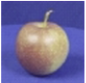
\includegraphics[width=0.8cm,height=0.8cm]{Images/deeper_look_apple.png}})$ = ``apple"}} \\[8pt]

	\hspace{4cm} \textcolor{blue}{\Huge{$f(\centering{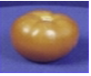
\includegraphics[width=0.8cm,height=0.8cm]{Images/deeper_look_tomato.png}})$ = ``tomato"}} \\[8pt]

	\hspace{4cm} \textcolor{blue}{\Huge{$f(\centering{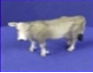
\includegraphics[width=0.8cm,height=0.8cm]{Images/deeper_look_cow.png}})$ = ``cow"}} 
\end{frame}


% Frame No: 3
\begin{frame}{Machine Learning Framework}

\hspace{2.5cm} \textbf{\Huge{\alert{y = f(x)}}} \\
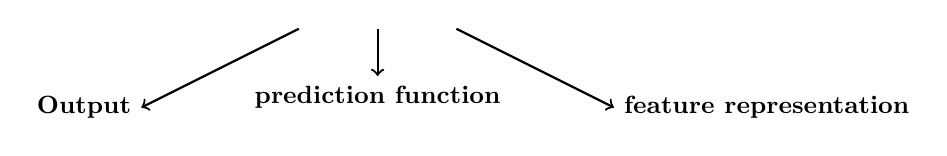
\begin{tikzpicture}
\draw[->, thick] (-1,3)--(-3,2) node[left]{\textbf{\small{Output}}};
\draw[->, thick] (0,3)--(0,2.4) node[below]{\textbf{\small{prediction function}}};
\draw[->, thick] (1,3)--(3,2) node[right]{\textbf{\small{feature representation}}};
\end{tikzpicture} \\

\begin{flushleft}
\textbf{\alert{Training:}} given a training set, estimate the prediction function \alert{$f$} by minimizing the prediction error \\[8pt]
\textbf{\alert{Testing:}} apply \alert{$f$} to never before seen test example \alert{$x$} and output predicted value \alert{$y = f(x)$}
\end{flushleft}
\end{frame}


% Frame No: 4
\begin{frame}{The Underlying Abstraction} 
\centering
\textsl{\alert{\Huge{$y = f(x)$}}}
\begin{itemize} \vspace{12pt}
\item What are \alert{$x,y$} for spam detection?
\item What are \alert{$x,y$} for image classification? 
\item What are \alert{$x,y$} for sentiment analysis?
\item What are \alert{$x,y$} for \textless insert your problem here\textgreater?
\end{itemize}
\end{frame}


% Frame No: 5
\begin{frame}{The Underlying Abstraction}
\centering
\textsl{\alert{\Huge{$y = f(x)$}}}
\begin{itemize} \vspace{12pt}
\item What are \alert{$f,x,y$} for the classification tasks? \vspace{4pt}
\item \alert{$x$} is often a vector (column matrix). \vspace{4pt}
\item \alert{$y$} is either 0 or 1 (binary) or \{1,2,...,p\} (multiclass) \vspace{4pt}
\end{itemize}
\end{frame}

% Frame No: 6
\begin{frame}{The Underlying Abstraction}
\centering
\textsl{\alert{\Huge{$y = f(w, x)$}}}
\begin{itemize} \vspace{12pt}
\item What is really \alert{$f()$}? \textsl{(This is what we need to find.)} \vspace{4pt}
\item Who gives \alert{$w$}? \textsl{(Data gives.)} \vspace{4pt}
\item Who gives the form of \alert{$f()$}? (eg. Quadratic, linear etc.?) \vspace{4pt}
\end{itemize}
\end{frame}

% Frame: 7 
\begin{frame}{Regression and Time Series}
	\only<3->{\vspace{0.21cm}}
	\only<2->{\alert{Regression}}
\begin{itemize}
	\item<2-> Predicting a real number is \vspace{0.5cm} regression
\end{itemize} %vspace{8pt}
	\only<3->{\alert{Time series Forecasting}}
\begin{itemize}
\item<3-> Predicting based on prior time tagged data
\end{itemize}
\end{frame}



% Frame: 8
{ 
\1
\begin{frame}
	\title{Training and Testing}
	\subtitle{Creating and Evaluating Models}
	\maketitle
\end{frame}
}

% Frame: 9
\begin{frame}
	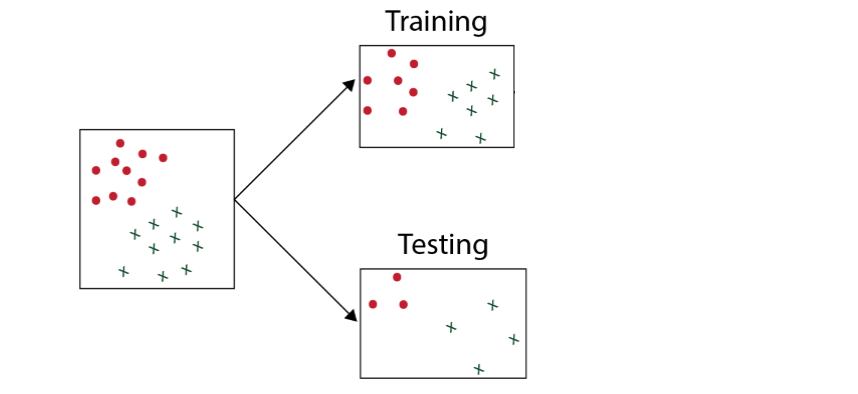
\includegraphics[width=0.9\textwidth, height=0.65\textheight]{Images/deeper_look_9.png}
\end{frame}

% Frame: 10
\begin{frame}[t]{Steps}
	\begin{itemize}
		\item Training
	\end{itemize}
	
	\begin{tikzpicture}
\transwipe<5,6,7>[duration=5]

		\only<1->{	\node[block,text width= 3.2cm, xshift=-5cm, yshift=0cm](b1){Training Data \\ 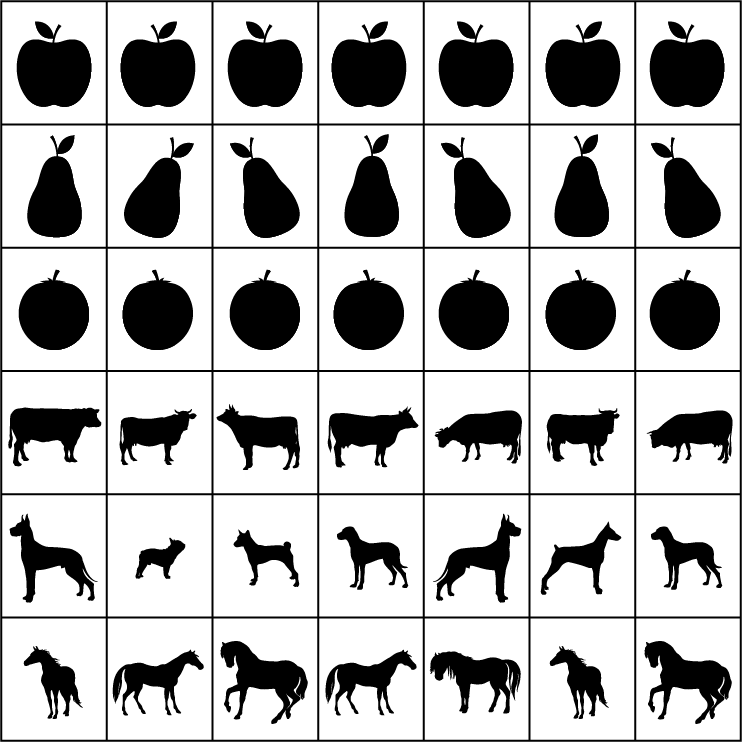
\includegraphics[width=3.2cm, height=3cm]{Images/deeper_look_10.png} };}
		\only<2->{	\node[block,right of =b1, xshift=2.5cm, yshift=0](b2){ Features \textcolor{white}{.....} };}
		\only<3->{	\node[block,right of= b2,xshift =1.5cm, yshift=0cm](b3){Training \textcolor{white}{..........}};}
		\only<3->{	\node[block,above of=b3, xshift=0cm, yshift=0.5cm](b4){Training Labels};}
		\only<4->{	\node[block,right of = b3, xshift = 1.7cm, yshift =0cm](b5){Learned Model};}
		%\only<4->{	\node[block, above of = b5, xshift = 0cm, yshift =0.5cm](b6){Validation data};}
		%\only<4->{	\node[block, below of = b5, xshift = 0cm, yshift=-0.5cm](b7){Validation Prediction};}
	
		\only<2-4>{	\draw[arrow] (b1) -- (b2);}
		\only<3-4>{	\draw[arrow] (b2) --(b3);}
		\only<3-4>{	\draw[arrow] (b4) -- (b3);}
		%\only<4-4>{	\draw[arrow] (b3) -- (b5);}
		%\only<4-4>{	\draw[arrow] (b6) -- (b5);}
		\only<4-4>{	\draw[arrow] (b3) -- (b5);}

		\only<4->{      \draw[arrow] (b2) --node[yshift=-1.1cm, xshift=-0.5cm, text width = 1.8cm, font = \scriptsize]{\textcolor{black}{- Prediction A}}(b3);}
	%	\only<5>{     \draw[arrow,cyan] (b1) -- (b2);}
         %       \only<5>{     \draw[arrow, cyan] (b2) --(b3);}
          %      \only<5>{     \draw[arrow,cyan] (b4) -- (b3);}
          %      \only<5>{     \draw[arrow, cyan] (b3) -- (b5);}
          %      \only<5>{     \draw[arrow, cyan] (b6) -- (b5);}
          %      \only<5>{     \draw[arrow, cyan] (b7) -- (b5);}


		\only<5->{      \draw[arrow] (b2) --node[yshift=-1.5cm, xshift=-0.5cm, text width = 1.8cm, font = \scriptsize]{\textcolor{black}{- Prediction B}}(b3);}
		\only<5>{     \draw[arrow,darkgray] (b1) -- (b2);}
                \only<5>{     \draw[arrow, darkgray] (b2) --(b3);}
                \only<5>{     \draw[arrow,darkgray] (b4) -- (b3);}
                %\only<5>{     \draw[arrow, darkgray] (b3) -- (b5);}
               % \only<5>{     \draw[arrow, darkgray] (b6) -- (b5);}
                \only<5>{     \draw[arrow, darkgray] (b3) -- (b5);}

		\only<6->{      \draw[arrow] (b2) --node[yshift=-1.9cm, xshift=-0.5cm, text width = 1.8cm, font = \scriptsize]{\textcolor{black}{- Prediction C}}(b3);}
		\only<6>{     \draw[arrow,green!50!cyan] (b1) -- (b2);}
                \only<6>{     \draw[arrow,green!50!cyan ] (b2) --(b3);}
                \only<6>{     \draw[arrow,green!50!cyan] (b4) -- (b3);}
               %\only<6>{     \draw[arrow, green!50!cyan] (b3) -- (b5);}
               %\only<6>{     \draw[arrow, green!50!cyan] (b6) -- (b5);}
                \only<6>{     \draw[arrow, green!50!cyan] (b3) -- (b5);}
		\only<7->{      \draw[arrow] (b2) --node[yshift=-2.3cm, xshift=-0.5cm, text width = 1.8cm, font = \scriptsize]{\textcolor{black}{- Prediction D}}(b3);}
		 \only<7>{     \draw[arrow,black] (b1) -- (b2);}
                \only<7>{     \draw[arrow, black] (b2) --(b3);}
                \only<7>{     \draw[arrow,black] (b4) -- (b3);}
               % \only<7>{     \draw[arrow, black] (b3) -- (b5);}
               % \only<7>{     \draw[arrow, black] (b6) -- (b5);}
                \only<7>{     \draw[arrow, black] (b3) -- (b5);}
		


		%		\only<9->{
%			\begin{blink}
%\draw[arrow] (b1) -- (b2);
%		\end{blink}}
	
	
	\end{tikzpicture}
\end{frame}


% Frame: 11
\begin{frame}[t]{Steps \ldots}
	\begin{itemize}
		\item Testing 
	\end{itemize}
	\begin{tikzpicture}
		\node[block, text width=0.9cm,text height=1cm,draw=white,  xshift=-5cm, yshift=0cm](n1){
\includegraphics[width=1.1cm, height=1.1cm]{Images/deeper_look_11.png}};
		\only<2->{	\node[block, xshift=-2.5cm, yshift = 0cm,text height=0.51cm](n2){\alert{Features \textcolor{white}{.....}}};}
		\only<3->{		\node[block, xshift=0.5cm, yshift=0cm, text height=0.51cm](n3){\alert{Learned model}};}
		\only<4->{\node[block, xshift=3.4cm, yshift=0cm, text height=0.51cm](n4){\alert{Prediction \textcolor{white}{....}}};}
		\only<2->{		\draw[arrow] (n1)--(n2);}
		\only<3->{		\draw[arrow] (n2)--(n3);}
		\only<4->{		\draw[arrow] (n3)--(n4);}
	\end{tikzpicture}
\end{frame}


% Frame: 12
\begin{frame}{Training and Testing}
\begin{itemize}
\item Training is the process of making the system able to learn
\item \alert{Assumptions:} \\
\setbeamertemplate{itemize items}[circle]
\begin{itemize}
\item Training set and testing set come from the same distribution
\item Need to make some assumptions or bias
\end{itemize}
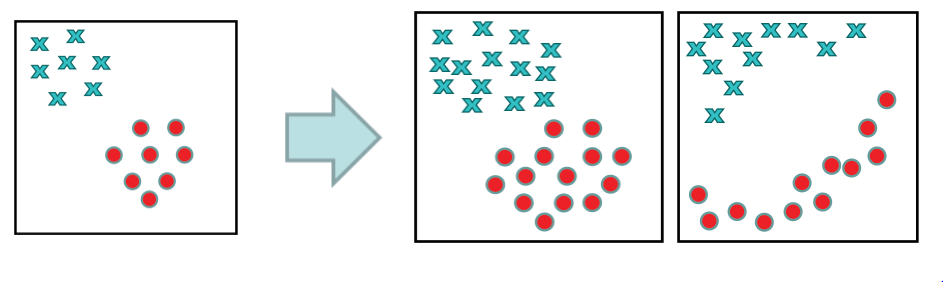
\includegraphics[width=10cm]{Images/deeper_look_12.png}
\end{itemize}
\end{frame}

% Frame: 13
\begin{frame}{Experiment}
	\begin{itemize}
		\item \href{https://drive.google.com/file/d/1mOFaciz7MuvR9oZ2tAEPwSPfCn-ljVzo/view?usp=sharing}{Demo\_Train\_test\_split\_Penguin} \\
			\begin{itemize}
				\item Dataset: Penguin \\
				\item Objective: To split the data into train and test sets using  train\_test\_split() from sklearn
			\end{itemize}
	\end{itemize}
\end{frame}

% Frame: 14
\begin{frame}[t]{ Two Prominent Learning Paradigms}
\begin{itemize}
\item \textbf{\alert{Supervised learning:}} It is the machine learning task of inferring a function from labeled training data  \vspace{12pt}
\item \textbf{\alert{Unsupervised Learning:}} Learn patterns from unlabeled data. Often look for a structure
\end{itemize}
\end{frame}

% Frame: 15
\begin{frame}{A ‘toy’ Classification Problem}
\begin{columns}
\column{0.75\textwidth}
\begin{itemize}
\item Apples vs Oranges
\item We have measured weight, color, sphericity
\item Some labeled data
\item Given unlabeled data decide which fruit it is\\[10pt]

\centering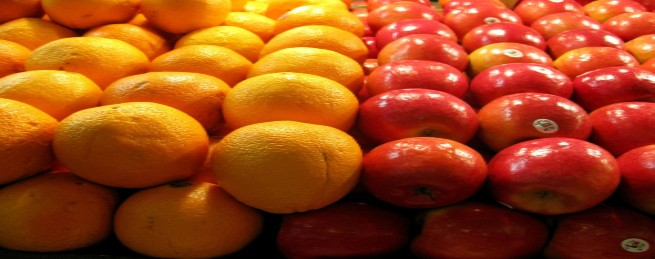
\includegraphics[width=0.75\textwidth, height=2.7cm]{Images/deeper_look_15.png}
\end{itemize}
\column{0.25\textwidth}
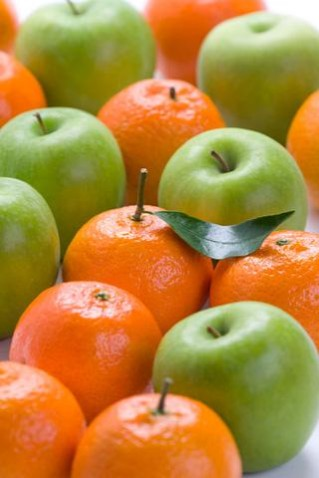
\includegraphics[width=0.9\textwidth,height=0.55\textheight]{Images/deeper_look_15a.png}
\end{columns}
\end{frame}

% Frame: 16
\begin{frame}{Visualizing a Sample in 2D}
\centering
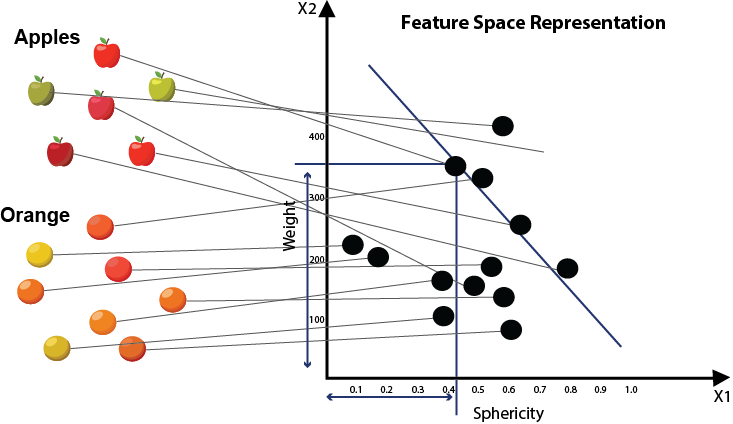
\includegraphics[width=0.8\textwidth,height=0.7\textheight]{Images/deeper_look_16.png}
\end{frame}


% Frame:17
\begin{frame}{Sample/Point and Representation}
\begin{itemize}
\item A sample is easy to visualize in 2D
      $\small x =  \left[\!
      \begin{array}{c}
      x_1 \\
      x_2
      \end{array}
      \!\right]$ \\
 \item And sometime in 3D with some effort  $ \small x =  \left[\!
      \begin{array}{c}
       x_1 \\
       x_2 \\
       x_3
      \end{array}
      \!\right]$ \\
\item And we often need much larger dimensionality in practice
    $ \small x =  \left[\!
    \begin{array}{c}
      x_1 \\
      x_2 \\
       . \\
      x_d
    \end{array}
  \!\right]$
\end{itemize}
\end{frame}




% Frame: 18
\begin{frame}[fragile]{Examples of Learned Function or Model}
\centering
$ \small x =  \left[\!
     \begin{array}{c}
      x_1 \\
      x_2 \\
       . \\
      x_{d}
      \end{array} 
      \!\right] w =  \left[\!
    \begin{array}{c}
      w_1 \\
      w_2 \\
       . \\
      w_d
      \end{array} 
	\!\right]$ \\[0.8cm]
$ w\cdot x = w_1 \cdot x_1 + w_2 \cdot x_2 + \ldots w_d \cdot x_d $ \vspace{1pt} \break

	\textbf{\large\textbf{ $ f(w,x) = sign(w \cdot x)$}}

\end{frame}



% Frame: 19
\begin{frame}{In General \ldots}
\centering
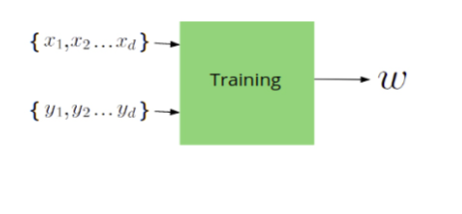
\includegraphics[width=0.7\textwidth,height=0.5\textheight]{Images/deeper_look_19.png} 
\end{frame}


% Frame: 20
\begin{frame}{Terminology}
	\begin{columns}
		\begin{column}{0.5\textwidth}
			\begin{itemize}
				\item Ground Truth
				\item Labels
				\item Predictions
				\item Training and Testing
				\item Supervised
				\item Unsupervised
			\end{itemize}
		\end{column}
		\begin{column}{0.5\textwidth}
			\begin{itemize}
				\item Features
				\item Input
				\item Output
				\item Feature Representation
				\item Samples
				\item Learning Model
				\item Classification
			\end{itemize}
		\end{column}
	\end{columns}
\end{frame}



\end{document}

